\documentclass[a4paper, oneside, 11pt, onecolumn]{article}

\usepackage{multirow}
\usepackage{graphicx}
\usepackage{subfigure}
\usepackage[round, comma, sort&compress, longnamesfirst]{natbib} 
\usepackage[left=2cm,top=3cm,right=1.5cm,bottom=2cm,bindingoffset=0.5cm]{geometry}
\usepackage{enumerate}
\usepackage{fancyhdr}
\pagestyle{fancy}
\fancyhead{}
\fancyfoot{}
\fancyfoot[L]{\textit{}}
 \fancyhead[L]{\textit{Clarke et al (20xx)}}
\renewcommand{\headrulewidth}{0.8pt}
\renewcommand{\footrulewidth}{0.8pt}
\setlength\headheight{14pt}
\fancyfoot[RO] {\thepage}
\usepackage{authblk}
%%%%%%%%%%%%

\begin{document}

\title{Supplementary Materials}

\author{A. D. F. Clarke\thanks{a.clarke@essex.ac.uk}}
 \affil{School of Psychology, University of Essex, UK}

\maketitle

\begin{abstract}

\end{abstract}

\section{Paradigm Details}


% These are the sizes of the boxes for each resolution, I'm not sure how best to incorporate this into the text though... here's a table for the meantime;
% Thanks! Stim size is not critical for our experiment, so it doesn't matter too much if it's too complicated (just habit to have it in there :)
\begin{table*}
	\centering
	\small
	\begin{tabular}{cc|c}
	    Experiment	    &	Resolution	     & Size of stim \\
		\hline
		Adaptive Choice & $1024 \times 768$  & $\approx$$1.8^{\circ}$ \\
		Adaptive Choice & $1400 \times 1050$ & $\approx$$1.3^{\circ}$ \\
		Adaptive Choice & $1600 \times 1200$ & $\approx$$1.1^{\circ}$ \\
		Foraging        & $1024 \times 768$  & $\approx$$1^{\circ}$ \\
		Foraging        & $1400 \times 1050$ & $\approx$$0.7^{\circ}$ \\
		Foraging        & $1600 \times 1200$ & $\approx$$0.6^{\circ}$ \\
	\end{tabular}
	\caption{Size of stimuli for each experiment and screen resolution}
	\label{tab:Screen_Res}
\end{table*}

\subsection{Split-half}

\subsection{Adaptive Choice}

The ACVS was based on the task described in \cite{irons-leber2016}, with a few changes [Or identical to the task described in Experiment 1 of Irons \& Leber, in press by then hopefully].

Each search display was composed of 54 small squares (size? What was viewing distance \& screen size?) arranged in three concentric rings around fixation, with 12, 18 and 24 items in the inner, middle and outer rings respectively. The inner ring was $XX^{\circ}$ and the outer ring was $XX^{\circ}$ from fixation. Of the 54 squares, 13 were red, 13 were blue, 14 were green and 14 were "variable". Variable distractors changes colours from trial-to-trial according to a cyclical pattern: the distractors would be red for 5 trials (called a "red plateau"), then across a period of 7 trials, they would change colour from almost red to magenta (at the fourth trial in the transition) to almost blue (see \cite{irons-leber2017}, for the specific colour values? Or supplemental?). The variable distractor would then be blue for 5 trials (blue plateau), and then transition back from almost blue through magenta to almost red. This 24-trial cycle would repeat throughout the entire experiment. 

A white digit appeared inside each square. Two targets - a red square and a blue square each with a digit between 2 and 5 - were embedded in every search display. The two target digits were always different, to enable us to distinguish the chosen target. The remaining red, blue and variable squares all contained digits between 6-9. Green squares could contain any digit between 2-9. The location of the targets and distractor within the search display were randomized on each trial.

Participants were informed that the search displays would contain two targets on every trial, that they need only find one target on each trial and that they were always free to search for either one. A trial began with a 1.5s ITI containing a central fixation cross, followed by the search display until a response was made. Participant responded by pressing a key that corresponded to the digit inside the target (\texttt{V}, \texttt{B}, \texttt{N} and \texttt{M} keys corresponding to 2, 3, 4 and 5 respectively). Participants completed 10 practice trials, followed by 3 blocks of 96 trials. Each block started on a red plateau.  


\subsection{Foraging}

The foraging task was based on \cite{kristjansson2014} and \cite{johannesson2016}. Participants completed the feature foraging and conjunction foraging tasks on separate days, with the order counterbalanced (was it counterbalanced?).

In the feature foraging task, search displays contained 80 small circles (size), 20 red (RGB: 180, 0, 0), 20 green (RGB: 20, 100, 40), 20 blue (RGB: 0, 0, 220) and 20 yellow (RGB: 200, 150, 0), presented against a black background. Stimuli were arranged in a 10 x 8 grid, but the position of each item within the grid space was jittered to create a more random spatial arrangement (with the restriction that two items could not be within 30 pixels of each other). The location of item colours to grid locations was completely randomized. 
For half of the participants, targets were red and green circles, and for the other half of participants, targets were blue and yellow circles. Participants were asked to collect all of the targets within a trial by using the mouse to click on each target. Clicking on a target caused it to disappear from the display. If the participant clicked erroneously on a non-target, the trial was immediately ended and a replacement trial was begun. Participants completed 1 practice trial and 20 full-completed experimental trials.

In the conjunction foraging task, search displays were composed of both circles and squares. For half of the participants, the shapes were red and green (equal numbers of red circles, red squares, green circles and green squares), and for the remaining participants the shapes were blue and yellow. Targets were defined by conjunctions of colour and shape (e.g., red squares and green circles, with red circles and green squares as distractors). The assignment of targets and distractors was assigned at random for each participant. The procedure was otherwise identical to the feature foraging task. 

%% For the assignment of distractors and targets, we generated a two lists of random numbers (1-2 for easy search, and 1-4 for hard search). Pretty sure we did that because counterbalancing became very tricky once you accounted for that as well. 

%%%%%%%%%%%%%%%%%%%%%%%%%%%%
\section{Participants}
%%%%%%%%%%%%%%%%%%%%%%%%%%%%

Data was collected from 64 participants as originally planned. Four of these participants did not complete all parts of the experiment (either declining to participate in the second session, or could not be calibrated with the eye tracker), so four new participants were recruited to bring the total back up to 64. 

\subsection{Split-Half}

Accuracy data from all participants is shown in Figure \ref{fig:splithalf_acc_all}. From this we can see that there are a number of outliers: 4, 21, 33, 56, and 58. These participants, in at least one session, either missed the majority of easy targets, or responded with false positives on the majority of target absent trials. After removing these participants, the lowest accuracy in either session was $84.6\%$ for the easy targets, and $76.9\%$ for target absent trials. This leaves us with 59 participants for the split-half paradigm. 

\begin{figure}
\centering
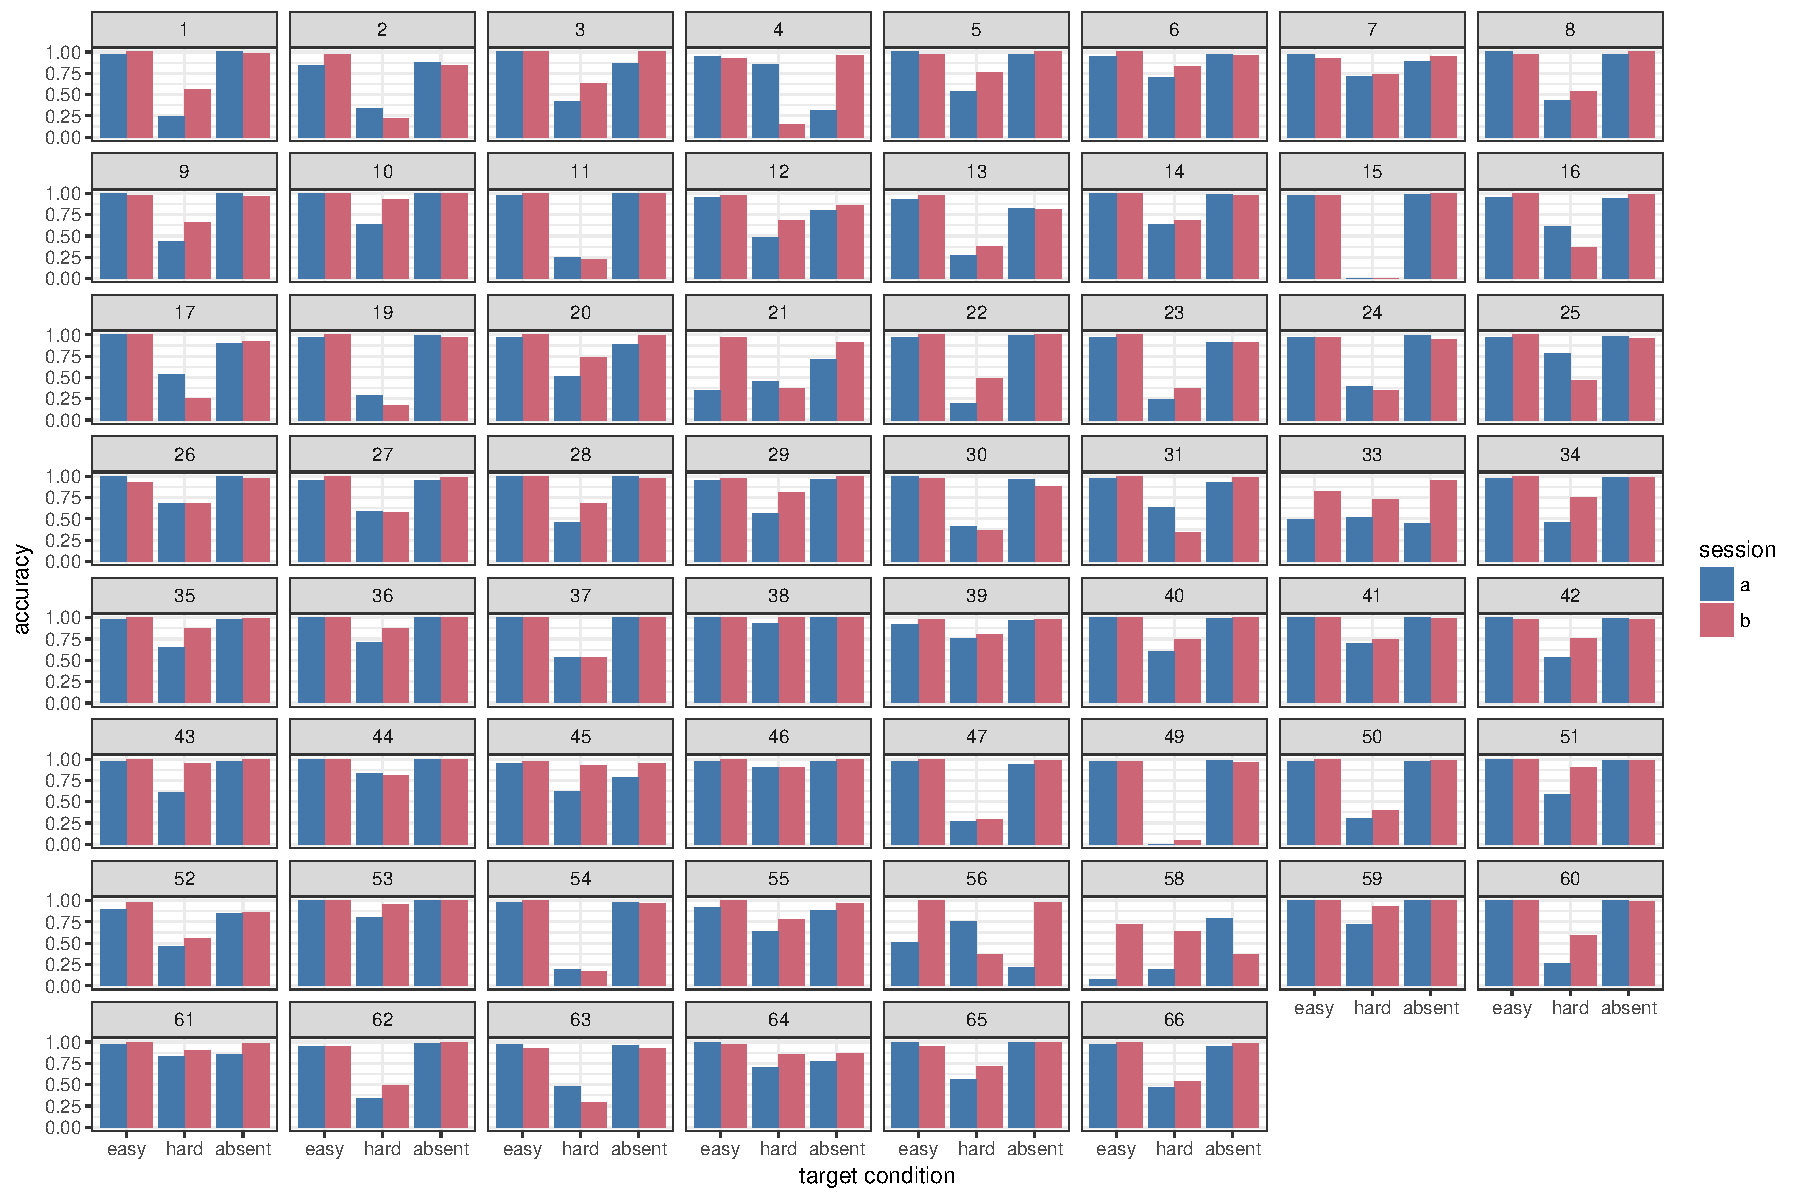
\includegraphics[width=14cm]{../Scripts/lineseg/scratch/acc_by_session_by_person.pdf}
\caption{Accuracy data for each participant for the split-half paradigm.}
\label{fig:splithalf_acc_all}
\end{figure}

\subsection{Adaptive Choice}

Two participants whose accuracy rates were more than 3 SD below the mean were removed from analyses, leaving 60 participants remaining for ACVS analyses. [REMOVED FOR ACCURACY: 38, 39. ALSO ONE PERSON MISSING AC DATA:32; THREE PEOPLE MISSING ALL DATA: 18, 48, 57]

\subsection{Foraging}

[ACCURACY OK BUT MISSING DATA: ONE PERSON MISSING MISSING CONJUNCTION DATA: 1; SIX PEOPLE MISSING FEATURE DATA: 31, 35, 49, 50, 51, 52; THREE PEOPLE MISSING ALL DATA: 18, 48, 57. TOTAL N = 56]

\subsection{Comparisons across paradigms}

Interestingly, it was not the same participants who had to be removed in each paradigm. This suggests that their poor performance in one paradigm is less likely to be due to low motivation. The number of participants available for each comparison between paradigms is given in Table \ref{tab:num_per_paradigm}.

\begin{table*}
\centering
\small
\begin{tabular}{cc|c}
 			&					& Number of participants\\
\hline
Split-half 	& Adaptive Choice 	& \\
Split-half 	& Foraging 			& \\
Adaptive Choice & Foraging 		& \\
\end{tabular}
\caption{Number of participants available for each comparison}
\label{tab:num_per_paradigm}
\end{table*}

\section{Data processing}

\subsection{Split-Half}

179 trials with invalid key responses were removed. After removing data from the five outlier participants (see above), all remaining incorrect trials ($n=2529$) were removed, leaving a total of 16187 trials over 59 participants.

\subsubsection{Reaction Times}
As expected, reaction times were highly skewed (Figure \ref{fig:splithalf_rt_dists_all}), so were $\log_2$ transformed (in ms units) before the participant means were calculated for each session and target condition (Figure )

\begin{figure}
\centering
\subfigure[]{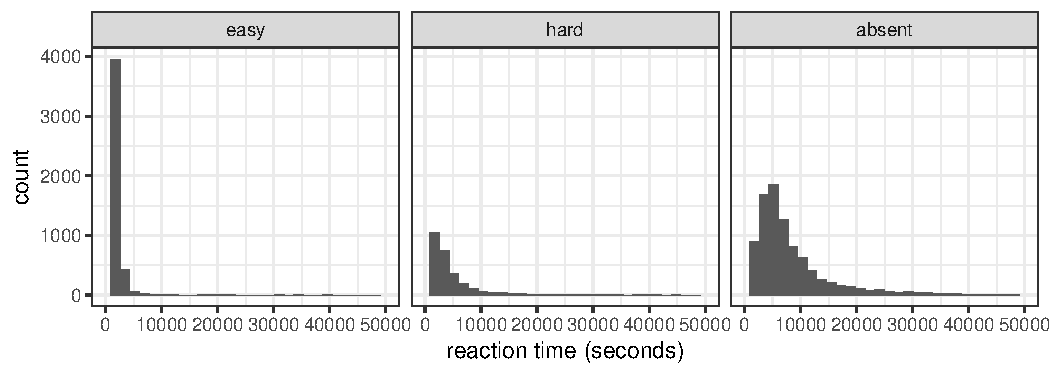
\includegraphics[width=14cm]{../Scripts/lineseg/scratch/rt_dists.pdf}}
\subfigure[]{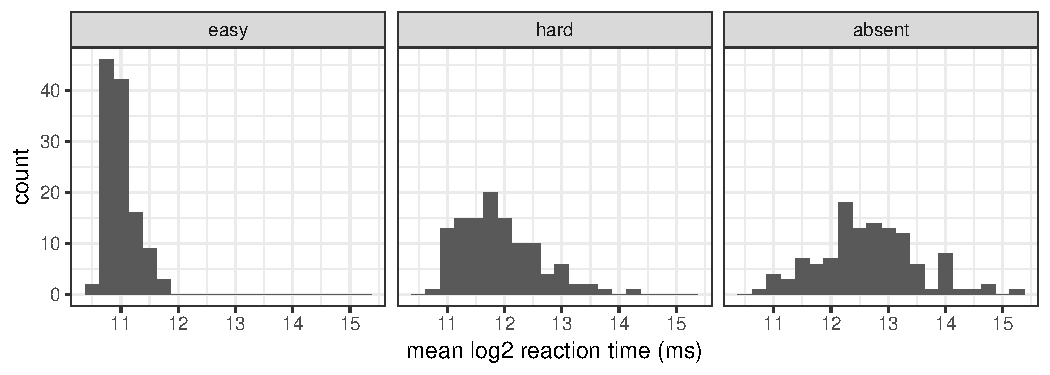
\includegraphics[width=14cm]{../Scripts/lineseg/scratch/rt_dists_mean.pdf}}
\caption{Distribution of reaction times in split-half paradigm.}
\label{fig:splithalf_rt_dists_all}
\end{figure}

\subsubsection{Eye movements}

340,138 fixations were recorded. Of these, 7701 fell outside of the stimuli area and were removed. Fixations landing within a vertical strip consisting of $10\%$ of the stimuli's width were classed as \textit{central}. All remaining fixations were then classed as landing on the \textit{homogeneous} or \textit{heterogeneous} half of the stimulus. Initial fixations were not included in the analysis. Numbers of fixations are given in Table \ref{tab:num_fix}.

\begin{table*}
\centering
\small
\begin{tabular}{c|c|r|r|r}
 		&	& $1<n$	& $2 \leq n \leq 5$ & $2 \leq n \leq 3$\\
\hline
\multirow{3}{*}{easy} 
& central		& 3931 	& 3689	& \\
& homogeneous 	& 12452	& 8312 	&\\
& heterogeneous & 5955	& 3241 	&\\
\hline
\multirow{3}{*}{hard} 
& central		& 3804 	& 2439	& \\
& homogeneous 	& 8781	& 3188	&	\\
& heterogeneous & 29912	& 5294	&\\
\hline
\multirow{3}{*}{absent} 
& central		& 16885 & 8303	& \\
& homogeneous 	& 41356	& 12576	&\\
& heterogeneous & 192348& 5763	&\\
\hline


\end{tabular}
\caption{Number of fixations recorded for each condition.}
\label{tab:num_fix}
\end{table*}

\subsection{Adaptive Choice}

[DON'T HAVE MUCH TO ADD HERE FOR EITHER ADAPTIVE CHOICE OR FORAGING THAT ISN'T ALREADY IN THE METHOD. BUT COULD SHIFT THAT INTO HERE IF YOU WANT]

\subsection{Foraging}



\end{document}


